%
% teil1.tex -- Beispiel-File für das Paper
%
% (c) 2020 Prof Dr Andreas Müller, Hochschule Rapperswil
%
% !TEX root = ../../buch.tex
% !TEX encoding = UTF-8
%

\section{Zustands- und Steuervariablen \label{leo:section:variabeln}}
\rhead{Zustands- und Steuervariablen}

Die Zustands- und Steuervariablen sind entscheidend für die Berechnung einer möglichst effizienten Flugbahn von der Erde in den Orbit. 
Sie beschreiben den aktuellen Zustand der Rakete und die Steuerungseingaben, die verwendet werden, um die gewünschte Flugbahn zu erreichen. 

Das Ziel ist es, zu jedem Zeitpunkt während des Aufstiegs die Position, Geschwindigkeit und Flugrichtung der Rakete zu kennen und kontrollieren zu können. 
Die Rakete startet senkrecht vom Boden (Meereshöhe) aus dem Stillstand und muss schließlich eine horizontale Flugrichtung sowie eine ausreichende Geschwindigkeit erreichen, um im Orbit zu bleiben. 

Die wichtigsten Zustands- und Steuervariablen sind:

\begin{itemize}
	\item \(\alpha\): Steuerungswinkel relativ zur momentanen Raketenrichtung (Pitch),
	\item \(\gamma\): Winkel der Flugrichtung relativ zum lokalen Horizont,
	\item \(v\): Maximal erreichbare Geschwindigkeit der Rakete,
	\item \(v_f\): Momentane Geschwindigkeit der Rakete,
	\item \(H\): Zielhöhe für den Orbit,
	\item \(h\): Momentane Höhe der Rakete relativ zum Startpunkt,
	\item \(m_0\): Anfangsmasse der Rakete inklusive Treibstoff,
	\item \(m_f\): Masse der Rakete ohne Treibstoff (Leermasse),
	\item \(t_f\): Zeit, bis die Rakete den Orbit erreicht,
	\item \(m\): Momentane Gesamtmasse der Rakete (ändert sich durch Treibstoffverbrauch).
\end{itemize}

In Abbildung\,\ref{fig:leo:forces} sind diese Zustands- und Steuervariablen anschaulich dargestellt, wie sie während des Aufstiegs wirken.

\begin{figure}
	\centering
	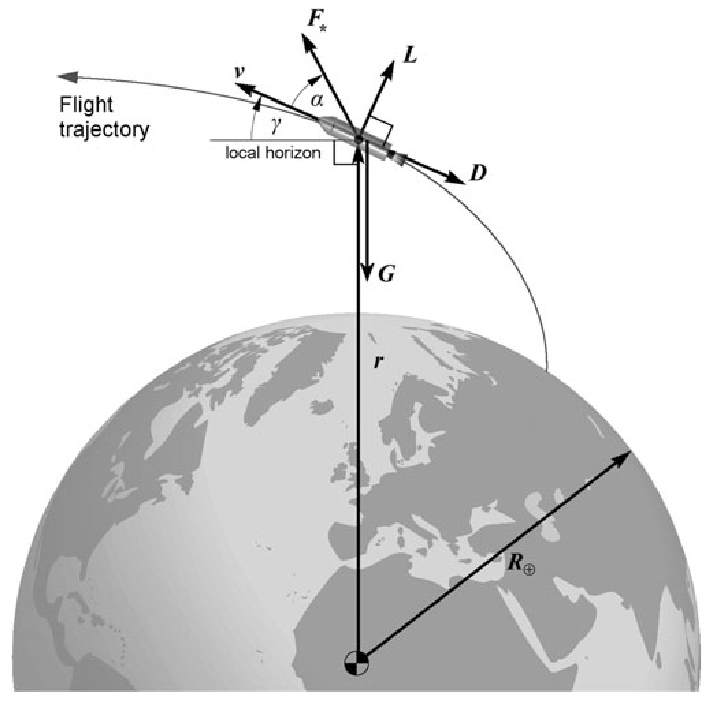
\includegraphics[width=0.5\linewidth]{papers/leo/Grafiken/forces.png}
	\caption{Zustands- und Steuervariablen veranschaulicht entnommen von \cite{leo:astronautics}.}
	\label{fig:leo:forces}
\end{figure}



\section{Bewegungsgleichungen und Raketenphysik \label{leo:section:beweungsgleichungen}}
\rhead{Bewegungsgleichungen und Raketenphysik}

Die Dynamik einer Rakete im Aufstieg zum Orbit wird durch eine Reihe von Differentialgleichungen beschrieben, die auf den grundlegenden physikalischen Gesetzen der Mechanik beruhen. 
Diese Gleichungen stellen das Kräftegleichgewicht dar, dem die Rakete unterliegt, und hängen von den Zustands- und Steuervariablen ab, die in Abschnitt \ref{leo:section:variabeln} eingeführt wurden. 
Die Bewegungsgleichungen, die in dieser Arbeit verwendet werden, basieren auf den ausführlichen Herleitungen aus \cite{leo:astronautics}, insbesondere aus dem Kapitel "Equations of Motion". 
Im Folgenden werden diese Gleichungen vereinfacht dargestellt, um ein grundlegendes Verständnis zu vermitteln.

\subsubsection{Geschwindigkeitsänderung \(\dot{v}\)}
Die Änderungsrate der Raketen-Geschwindigkeit während des Aufstiegs ist durch die Gleichung
\[
\dot{v} = \frac{F_*}{m} \cos \alpha - \frac{D}{m} - g \sin \gamma
\]
gegeben, wobei:
\begin{itemize}
	\item \(\dot{v}\) die Beschleunigung der Rakete in Flugrichtung ist,
	\item \(F_*\) der Schub ist, den die Rakete durch ihre Triebwerke erzeugt,
	\item \(m\) die aktuelle Masse der Rakete ist, die durch den Treibstoffverbrauch ständig abnimmt,
	\item \(\alpha\) der Steuerungswinkel ist, der beschreibt, wie viel der Schubkraft tatsächlich für die Beschleunigung in Flugrichtung genutzt wird,
	\item \(D\) der Luftwiderstand ist, der der Vorwärtsbewegung entgegenwirkt,
	\item \(g \sin \gamma\) die Gravitationskraftkomponente ist, die der Bewegung entgegenwirkt, abhängig vom Winkel \(\gamma\) zum Horizont.
\end{itemize}
Diese Gleichung beschreibt die Netto-Beschleunigung der Rakete, indem der Schub gegen die widerstehenden Kräfte, wie Luftwiderstand und Schwerkraft, abgewogen wird. 
Der Steuerungswinkel \(\alpha\) beeinflusst, wie effektiv der Schub in Vorwärtsbewegung umgewandelt wird.

\subsubsection{Änderung des Flugwinkels \(\dot{\gamma}\)}
Die Änderung des Flugwinkels \(\gamma\), der den Winkel der Rakete zum lokalen Horizont beschreibt, ist durch die Gleichung
\[
\dot{\gamma} = \frac{1}{v}\left( \frac{F_*}{m} \sin \alpha + \frac{L}{m} - \left(g - \frac{v^2}{r}\right) \cos \gamma \right)
\]
gegeben, wobei:
\begin{itemize}
	\item \(\dot{\gamma}\) die Änderungsrate des Flugwinkels ist,
	\item \(L\) der Auftrieb ist, der durch aerodynamische Kräfte auf die Rakete wirkt,
	\item Der Term \(\left(g - \frac{v^2}{r}\right) \cos \gamma\) beschreibt die Kombination von Gravitationskräften und Zentripetalkraft, die durch die Bewegung der Rakete erzeugt wird.
\end{itemize}
Diese Gleichung beschreibt das Pitch-Manöver, bei dem die Rakete durch Schubvektorkontrolle und aerodynamische Kräfte ihre Ausrichtung relativ zum Horizont ändert. Das Manöver beginnt üblicherweise nach der Startphase, sobald die Rakete eine ausreichende Höhe erreicht hat, um die atmosphärischen Einflüsse zu reduzieren.

\subsubsection{Vertikale Position \(\dot{h}\)}
Die Änderungsrate der Höhe der Rakete ist durch die Gleichung
\[
\dot{h} = v \sin \gamma
\]
gegeben. 
Diese beschreibt, wie schnell die Rakete an Höhe gewinnt, basierend auf ihrer momentanen Geschwindigkeit \(v\) und ihrem Flugwinkel \(\gamma\). 
Je näher \(\gamma\) an 90° liegt, desto steiler ist der Flug und desto schneller steigt die Rakete vertikal auf.

\subsubsection{Horizontale Position \(\dot{x}\)}
Die horizontale Bewegung der Rakete wird durch die Gleichung
\[
\dot{x} = v \cos \gamma
\]
beschrieben, wobei \(v \cos \gamma\) die horizontale Komponente der Geschwindigkeit ist. 
Diese Gleichung stellt sicher, dass die Rakete nicht nur in der Höhe, sondern auch horizontal vorwärts bewegt wird, was entscheidend für das Erreichen der Umlaufgeschwindigkeit ist.

\subsection{Vereinfachte Herleitung der Bewegungsgleichungen}
Die Herleitung dieser Gleichungen basiert auf den grundlegenden Prinzipien der Newton'schen Mechanik. Für eine Rakete, die in die Atmosphäre startet und sich in den Weltraum bewegt, gelten folgende Überlegungen:

\begin{enumerate}
	\item \textbf{Kräftegleichgewicht}: Die resultierende Kraft, die auf die Rakete wirkt, ist die Summe der Schubkraft \(F_*\), der Luftwiderstandskraft \(D\) und der Schwerkraft \(g\). 
	Diese Kräfte beeinflussen sowohl die Geschwindigkeit als auch die Richtung der Rakete.
	
	\item \textbf{Masseänderung}: Die Rakete verliert kontinuierlich Masse durch den Treibstoffverbrauch. 
	Dieser Masseverlust führt zu einer Zunahme der Geschwindigkeit, die durch die Raketengleichung von Tsiolkovsky beschrieben wird.
	
	\item \textbf{Steuerung durch Pitch-Manöver}: Das Pitch-Manöver wird durch den Steuerungswinkel \(\alpha\) eingeleitet, der den Schubwinkel zur Flugrichtung bestimmt. 
	Ein kleiner Steuerungswinkel reduziert die Schubkomponente in der Vertikalrichtung, was der Rakete ermöglicht, ihre Flugbahn zu kippen und eine stabile Umlaufbahn zu erreichen.
\end{enumerate}

Die Bewegungsgleichungen sind daher eine direkte Folge des Kräftegleichgewichts, kombiniert mit der dynamischen Masseänderung und der Schubsteuerung. 
Sie ermöglichen es, die Raketenflugbahn präzise zu berechnen und gleichzeitig die Steuerungsparameter zu optimieren.


\subsection{Orbit \label{leo:orbit}}
Ein Raumfahrzeug in einem Orbit um einen Planeten verhält sich ähnlich wie ein geschwungener Gegenstand an einer Kette. 
Die notwendige Geschwindigkeit, damit ein Raumfahrzeug in einer stabilen Umlaufbahn bleibt, lässt sich berechnen mit:
\[
v = \sqrt{\frac{\mu}{r}},
\]
wobei \(r\) der Radius vom Mittelpunkt des Planeten bis zur Rakete und \(\mu\) der Gravitationsparameter des Planeten ist. 
Für die Erde beträgt der Gravitationsparameter \(\mu_{Erde} = GM_{Erde} = 3.99 \times 10^5 \, km^3/s^2\). Raumfahrzeuge in niedrigen Umlaufbahnen (Low Earth Orbit, LEO), wie etwa die Internationale Raumstation (ISS), befinden sich typischerweise in einer Höhe von etwa 400\,km und benötigen eine Geschwindigkeit von etwa \(7.67 \, km/s\), um im Orbit zu bleiben.

\subsection{Schwerkraft}
Die Schwerkraft ist eine der größten Kräfte, die eine Rakete während des Aufstiegs überwinden muss. 
Sie nimmt mit zunehmender Höhe ab, aber die Rakete muss genügend Geschwindigkeit aufbauen, um der Schwerkraft dauerhaft zu entkommen und eine stabile Umlaufbahn zu erreichen. 
Die Schwerkraft bremst die Rakete ab, was durch folgende Gleichung beschrieben wird:
\[
v_g = \int_0^t g \sin(\gamma) \, dt,
\]
wobei \(g\) die Gravitationskraft und \(\gamma\) der Flugwinkel ist. 
Entscheidend ist, ob die Rakete den Schub direkt gegen die Schwerkraft ausübt, was in der Berechnung der Flugbahn berücksichtigt wird.

\subsection{Atmosphäre}
Der Luftwiderstand \(D(t)\), der auf die Rakete wirkt, ist abhängig von der Geschwindigkeit sowie der Luftdichte. 
Die Luftdichte \(\rho(y)\) nimmt mit der Höhe \(y\) ab. Der Luftwiderstand lässt sich mit folgender Gleichung berechnen:
\[
D(t) = \frac{1}{2} \rho(y(t)) C_d A v^2(t),
\]
wobei \(C_d\) der Luftwiderstandsbeiwert und \(A\) die Querschnittsfläche des Fahrzeugs ist. 
Der Luftwiderstand ist besonders in den dichten Schichten der Atmosphäre relevant und nimmt mit steigender Höhe ab. 
Dieser Strömungsverlust kann in Form einer Geschwindigkeit \(v_l\) ausgedrückt werden:
\[
v_l = \frac{1}{H} \int_0^{t_f} k_D v^2 e^{-\frac{h}{H}} \, dt,
\]
wobei \(H\) eine charakteristische Höhe und \(k_D\) ein konstanter Strömungskoeffizient ist.


